\documentclass{scrartcl}
\usepackage[utf8]{inputenc}
\usepackage{graphicx}%GRaphiken
\usepackage{tabularx}%Tabellen!
\usepackage{url}% Urls besser
\usepackage{textcomp}% Sonderzeichen
\usepackage{amsmath}%maths / equations
\usepackage{booktabs} % for cmidrule
\usepackage{todonotes}
\usepackage[
	left=3cm,
	right=2cm,
	top=1.5cm,
	bottom=1cm,
	includeheadfoot
	]{geometry}														% Satzspiegel
\usepackage[
	round,	%(defaultage in the main file and \input ) for round parentheses;
	%square,	% for square brackets;
	%curly,	% for curly braces;
	%angle,	% for angle brackets;
	colon,	% (default) to separate multiple citations with colons;
	%comma,	% to use commas as separaters;
	authoryear,% (default) for author-year citations;
	%numbers,	% for numerical citations;
	%super,	% for superscripted numerical citations, as in Nature;
	sort,		% orders multiple citations into the sequence in which they appear in the list of 				references;
	%sort&compress,    % as sort but in addition multiple numerical citations
                   % are compressed if possible (as 3-6, 15);
	%longnamesfirst,  % makes the first citation of any reference the equivalent of
                   % the starred variant (full author list) and subsequent citations
                   %normal (abbreviated list);
	%sectionbib,      % redefines \thebibliography to issue \section* instead of \chapter*;
                   % valid only for classes with a \chapter command;
                   % to be used with the chapterbib package;
	%nonamebreak,     % keeps all the authors names in a citation on one line;
                   %causes overfull hboxes but helps with some hyperref problems.
]{natbib}											    			% Literaturverzeichnis
\usepackage[pdfpagelabels,plainpages=false, pageanchor=false]{hyperref}	


%% andere Einstellungen
\linespread{1.5}% 1.5 Zeilenabstand			


%% ----------------------------------------------------------------------------
\title{Ecotoxicology is not normal.}
\subtitle{How the use of proper statistical models can increase statistical power in ecotoxicological experiments.}
\author{Eduard Szöcs, Ralf B. Schäfer}
\date{\today}



%% ----------------------------------------------------------------------------
\begin{document}
\maketitle

%% ----------------------------------------------------------------------------
\section*{Abstract}
Ecotoxicologists are often confronted with non-normally distributed data.
To meet the assumptions of normality and heteroscedasticity, the standard procedure has been to either transform the data or use non-parametric methods if this fails.
Here, we compare the statistical power of analyses using transformed data or non-parametric methods to analyses using appropriate distributional assumptions, namely Generalised Linear Models (GLM).

We simulated data mimicking ecotoxicological experiments of two common data types (counts and proportions). 
We compare the performance of methods in terms of statistical power and type 1 error.
In addition, we outlined differences and advantages of GLMs on a real world mesocosm data set.

We found that GLMs provide in most cases a gain in statistical power compared to analysis of transformed data or using non-parametric methods.
We recommend that non-normal data should be analysed by GLMs and not by transformations or non-parametric methods.
GLMs should become a standard method in ecotoxicology. 





%% ----------------------------------------------------------------------------
\section{Introduction}
\label{sec:intro}
Ecotoxicologists perform various kinds of experiments yielding different types of data.
Examples are: animal counts in mesocosm experiments (positive, integer-valued data), proportions of surviving animals (data bonded between 0 and 1, continuous) or biomass in growth experiments (positive, continuous data).
These data are typically not normally distributed. 
Nevertheless, they are usually analysed using methods assuming a normal distribution and variance homogeneity \citep{wang_making_2011}. 
To meet these assumptions, data are usually transformed.
For example, ecotoxicological textbooks \citep{newman_quantitative_2012} and guidelines \citep{epa_methods_2002,oecd_current_2006} advise that survival data can be transformed using an arcsine square root transformation. 
For count data from mesocosm experiments a log(Ay + C) transformation is usually applied, where the constants A and C are either chosen arbitrarily or following general recommendations. 
For example, \citet{van_den_brink_impact_2000} suggest to set the term Ay to be 2 for the lowest abundance value (y) greater than zero and C to 1. 
Moreover, other transformations like the square root or fourth root are commonly applied in community ecology.
Note that there has been little evaluation and advice for practitioners, which transformations to use.
If the transformed data still do not meet the assumptions (i.e. normality and variance homogeneity), non-parametric tests are usually applied \citep{wang_making_2011}.

Generalised linear models (GLM) provide a method to analyse such non-normally distributed data \citep{nelder_generalized_1972}.
GLMs can handle various types of data distributions, e.g. Poisson or negative binomial (for count data) or binomial (for proportions); the normal distribution being a special case of GLMs.
Despite GLMs being available more than 40 years, ecotoxicologists do not regularly make use of them.
Recent studies concluded that data transformations should be avoided and GLMs be used as they have better statistical properties \citep{ohara_not_2010, warton_arcsine_2011}. 

Ecotoxicological experiments often involve small sample sizes due to practical constraints. 
For example, extremely low samples sizes (n \textless 5) are common in many mesocosm studies \citep{sanderson_pesticide_2002,szocs_analysing_2015}.
Small sample sizes lead to low power in statistical hypothesis testing, on which many ecotoxiological approaches (e.g. risk assessment for pesticides) rely. 
Such an endpoint are L/NOEC (Lowest / No observed effect concentration) values.
Although their use has been heavily criticized in the past \citep{laskowski_good_1995},  they are still regularly used in ecotoxicology \citep{jager_bad_2012}.
Especially in mesocosm studies L/NOEC calculations are used in the majority of mesocosm experiments \citep{brock_minimum_2015, efsa_ppr_guidance_2013}. 

We explore how GLMs may enhance inference in ecotoxicological studies and compared three types of statistical methods (transformation and normality assumption, GLM, non-parametric tests).
We first illustrate differences between statistical methods using a data set from a mesocosm study.
Then we further elaborate differences in detecting a general treatment effect and determining the LOEC using simulations of two common data types in ecotoxicology: counts and proportions. 



%% ----------------------------------------------------------------------------
\section{Methods}
\label{sec:methods}

%% --------------------------------
\subsection{Models for count data}
\subsubsection{Linear model for transformed data}
To meet the assumptions of the standard linear model, count data usually needs to be transformed. 
We followed the recommendations of \citet{van_den_brink_impact_2000} and used a log(Ay + 1) transformation (eqn. \ref{eqn:trans}):

\begin{align}
  y^T_i & = log(Ay_i + 1) \label{eqn:trans} \\
  A & = 2~/~min(y)~~~\text{, for}~ y > 0 \nonumber
\end{align}

, where $y_i$ is the measured abundance and $y_i^T$ the transformed abundance. 

Then we fitted the linear model to the transformed abundances (hereafter $LM$):

\begin{align}
  y_i^T &\sim N(\mu_i, \sigma^2) \nonumber \\
  y_i^T &= \alpha + \beta x_i \label{eqn:normal} \\
  var(y_i^T) &= \sigma^2 \nonumber
\end{align}

This model assumes a normal distributed response with constant variance ($\sigma^2$).
Note, that we parameterised the model as contrast ($\beta x_i$) to the control group ($\alpha$) so that parameters ($\beta$) are directly interpretable as changes from the control group (eqn. \ref{eqn:normal}).


\subsubsection{Generalised Linear Models}
GLMs extend the normal model by modelling other distributions.
Instead of transforming the response variable, the counts could be directly modelled by a Poisson distribution ($GLM_p$):

\begin{align}
  y_i &\sim P(\lambda_i) \nonumber \\
  log(\lambda_i) &= \mu_i \label{eqn:pois} \\
  \mu_i &= \alpha + \beta x_i \nonumber \\
  var(y_i) &= \lambda_i \nonumber
\end{align}

Again, this model was parametrised as contrast to the control group. 
The response variable is linked to the predictors via a log-function to avoid negative fitted values (eqn. \ref{eqn:pois}). 
The Poisson distribution assumes that mean and variance are equal - an assumption that is rarely met with ecological data, which is typically characterized by greater variance than the mean (overdispersion).
To overcome this problem a quasi-Poisson distribution could be used which introduces an additional overdispersion parameter ($\Theta$) ($GLM_{qp}$, eqn. \ref{eqn:quasi}).

\begin{align}
  y_i &\sim P(\lambda_i, \Theta) \label{eqn:quasi} \\
  var(y_i) &= \Theta \lambda_i  \nonumber
\end{align}

The quasi-Poisson model yields to parameter estimates equal to the Poisson model (eqn. \ref{eqn:pois}), but with standard errors scaled by the degree of overdispersion.

Another possibility to deal with overdispersion is to fit a negative binomial distribution ($GLM_{nb}$, eqn. \ref{eqn:negbin}).

\begin{align}
  y_i &\sim NB(\lambda, \kappa) \label{eqn:negbin}  \\
  var(y_i) &= \lambda_i + \kappa \lambda_i^2 \nonumber
\end{align}

In both cases the parametrisation and link function is equal to the Poisson GLM (eqn. \ref{eqn:pois}).
Note, that the quasi-Poisson model assumes a linear mean-variance relationship (eqn. \ref{eqn:quasi}), whereas the negative binomial model assumes a quadratic relationship (eqn. \ref{eqn:negbin}).

The above described models are most commonly used in ecology \citep{ver_hoef_quasi-poisson_2007}, although other distributions for count data are possible, like the negative binomial model with a linear mean-variance relationship (also known as NB1) or the poisson inverse gaussian model \citep{hilbe_modeling_2014}.


\subsection{Models for binomial data}
\subsubsection{Linear model for transformed data}
To accommodate the assumptions for the standard linear model, a special arcsine square root transformation (eqn. \ref{eqn:arcsine}) is suggested for such  data \citep{epa_methods_2002,newman_quantitative_2012}:

\begin{align}
  y_i^T = 
  \begin{cases}  
    arcsin(1) - arcsin(\sqrt{\frac{1}{4n}}) & \text{, if}\ y_i = 1 \\
    arcsin(\sqrt{\frac{1}{4n}}) & \text{, if}\ y_i = 0  \\
    arcsin(\sqrt{y_i}) & \text{, otherwise}
  \end{cases} \label{eqn:arcsine}
\end{align}

, where $y_i^T$ are the transformed proportions and n is the number of exposed animals per treatment ($n = 4 \cdot 10=40$).
The transformed proportions are then analysed using the standard linear model ($LM$, eqn. \ref{eqn:normal}).
Note, that the parameters of the linear model are not directly interpretable due to transformation.


\subsubsection{Generalised Linear Models}
Data of type \emph{x out of N} can be modelled by a binomial distribution with parameters N and $\pi$ ($GLM_{bin})$:

\begin{align}
  y_i &\sim Bin(N, \pi_i) \nonumber \\
  logit~(\pi_i) &= \alpha + \beta x_i \label{eqn:bin} \\
  var(y_i) &=  \pi_i (1 - \pi_i) / N \nonumber
\end{align}

, where N = number of exposed animals and $\pi$ is the probability of survival.
The variance of the binomial distribution is a quadratic function of the mean (eqn. \ref{eqn:bin}).
The parameters $\beta$ of this model are directly interpretable as changes in log odds compared to the control group.
Note, that there are also quasi-binomial models available if the assumed mean-variance relationship is not met. 


%% --------------------------------
\subsection{Statistical Inference}
After model fitting and parameter estimation the next step is statistical inference.
Ecotoxicologists are generally interested in two hypotheses: (i) is there any treatment related effect? and (ii) which treatments show a treatment effect (to determine the LOEC)?

Following general recommendations \citep{bolker_generalized_2009,faraway_extending_2006}, we used F-tests ($LM$ and $GLM_{qp}$) and Likelihood-Ratio (LR) tests ($GLM_p$, $GLM_{nb}$ and $GLM_{bin}$) to test the first hypothesis.
However, it is well known that LR test are unreliable with small sample sizes \citep{wilks_large-sample_1938}.
Therefore, we additionally explored parametric bootstrap \citep{faraway_extending_2006} to assess the significance of the LR.
Bootstrapping is computationally very intensive and for this reason we applied it only for the negative binomial models (using 500 bootstrap samples, denoted as $GLM_{npb}$).

To assess the LOEC we used Dunnett contrasts with one-sided Wald t tests (normal and quasi-Poisson models) and one-sided Wald Z tests (Poisson, negative binomial and binomial models).
Beside these parametric methods we also applied two, in ecotoxicology commonly used, non-parametric methods: The Kruskal-Wallis test  ($KW$) to test for a general treatment effect and a pairwise Wilcoxon test ($WT$) to determine the LOEC.



%% --------------------------------
\subsection{Case study}
\citet{brock_minimum_2015} presents a typical example of data from mesocosm studies, which we use to demonstrate differences between methods.
The data are mayfly larvae counts on artificial substrate samplers were at one sampling date. 
A total of 18 mesocosm have been sampled from 6 treatments (Control (n = 4), 0.1, 0.3, 1, 3 mg/L (n = 3) and 10 mg/L (n = 2)) (Figure \ref{fig:example}).

\begin{figure}
  \centering
  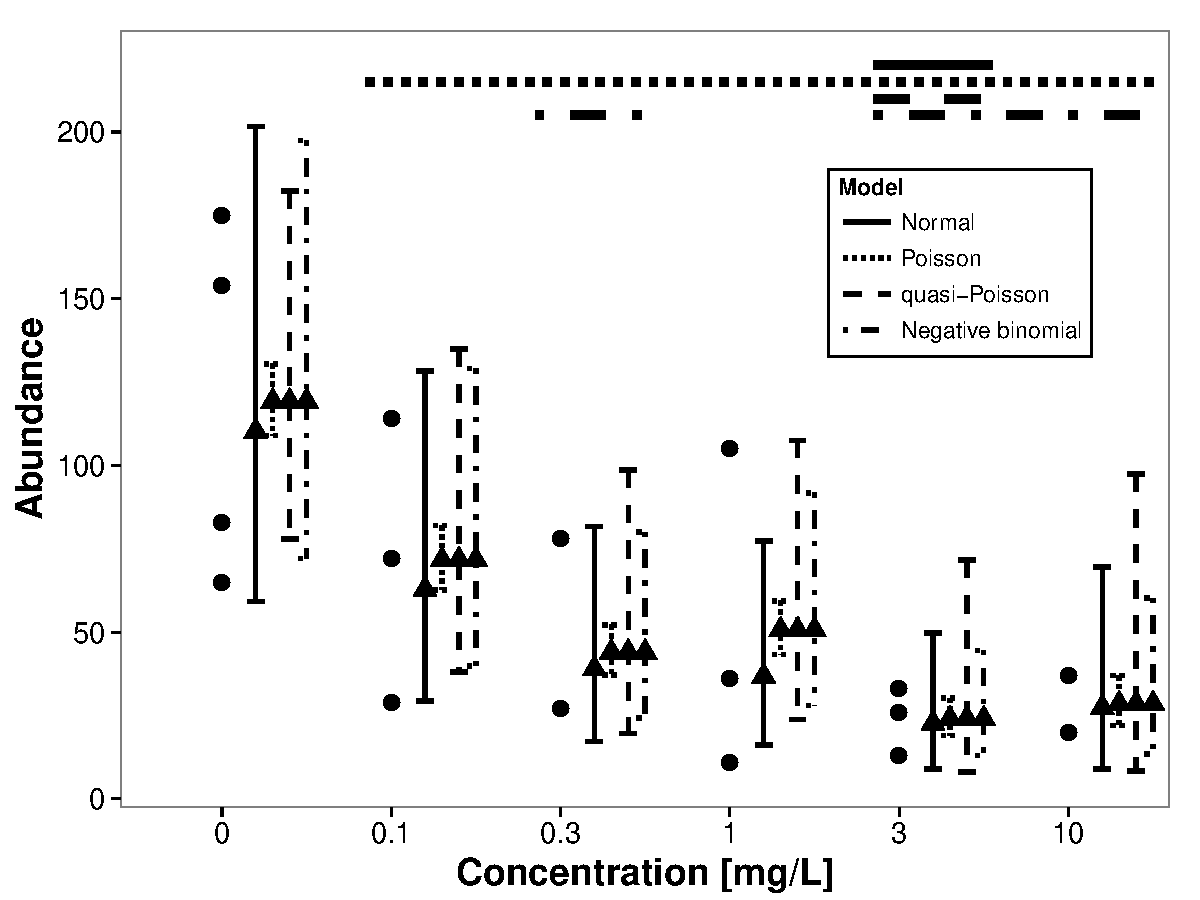
\includegraphics[width = 0.7\textwidth]{example.pdf}
  \caption{Data from \citet{brock_minimum_2015} (dots). 
  Predicted values (triangles) and 95\% Wald Z or t confidence intervals from the fitted models (vertical lines) are given beside.
  Horizontal bars above indicate treatments statistically significant different from the control group (Dunnett contrasts).
  The data showed considerable overdispersion ($\Theta = 22.41$) and therefore, the Poisson model underestimates the confidence intervals.
  }
  \label{fig:example}
\end{figure}


%% --------------------------------
\subsection{Simulations}
\subsubsection{Count data}
To further scrutinise the differences between methods we simulated data sets with known properties.
We simulated count data that mimics the data of the case study with five treatments (T1 - T5) and one control group (C).
Counts were drawn from a negative binomial distribution with slight over dispersion at all treatments ($\kappa = 0.25$, eqn. \ref{eqn:negbin}).
We simulated data sets with different number of replicates (N = \{3, 6, 9\}) and different abundances in control treatments ($\mu_\text{\tiny C}$ = \{2, 4, 8, 16, 32, 64, 128\}). 
For power estimation, mean abundance in treatments T2 - T5 was reduced to half of control and T1 ($\mu_\text{\tiny T2}~=~...~=~\mu_\text{\tiny T5}~=~0.5~\mu_\text{\tiny C} = 0.5~\mu_\text{\tiny T1}$), resulting in a theoretical LOEC at T2.
Mean abundance was kept equal between all groups in Type 1 error simulations.

We generated 100 data sets for each combination of N and $\mu_\text{\tiny C}$ and analysed these using the models outlined previously.
We did not fit Poisson models because we simulated data with overdispersion.


\subsubsection{Binomial data}
We simulated data from a commonly used design as in \citep{weber_short-term_1989}, with 5 treated (T1 - T5) and a control group (C). 
Proportions were drawn from a Bin(10, $\pi$) distribution, with varying probability of survival ($\pi$ = \{0.60, 0.65, 0.70, 0.75, 0.80, 0.85, 0.90, 0.95\}) and varying number of replicates (N = \{3, 6, 9\}).
For Type 1 error estimation, $\pi$ was held constant between groups.
For power estimation $\pi$ in C and T1 was fixed at 0.95 and was set to values between 0.6 and 0.95 for the treatments T2 - T5. 
For each combination we simulated 250 data sets. 

\subsection{Data Analysis}
We analysed the case study and the simulated data using the outlined methods.
We compared the methods and models in terms of Type 1 error (maintain a significance level of 0.05 when there is no effect) and power (detect an effect when it is present).
All computations were done in R (Version 3.1.2) \citep{r_core_team_r:_2014} on a Linux machine.
Source code for the simulations and analysis of the case study is available online at \url{https://github.com/EDiLD/usetheglm}.



%% ----------------------------------------------------------------------------
\section{Results}
\label{sec:results}
%% --------------------------------
\subsection{Case study}
The data set showed considerable overdispersion ($\Theta = 22.41$, eqn. \ref{eqn:quasi}).
Therefore, the Poisson model did not fit to this data and lead to underestimated standard errors and confidence intervals, as well as overestimated statistical significance (Figure \ref{fig:example}).
In this case, inferences on the Poisson model are not valid and we do not further discuss its results.
The normal (F = 2.57, p = 0.084) and quasi-Poisson model (F = 2.90, p = 0.061), as well as the Kruskal test (p =  0.145) did not show a statistically significant treatment effects.
By contrast, the LR test and parametric bootstrap of the negative binomial model indicated a treatment-related effect (LR = 13.99, p = 0.016, bootstrap: p = 0.042).

All methods predicted similar values, except the normal model predicting always lower abundances (Figure \ref{fig:example}). 
95\% confidence intervals (CI) where most narrow for the negative binomial model and widest for the quasi-Poisson model - especially at lower estimated abundances.
Consequently, the LOECs differed (Normal and quasi-Poisson: 3 mg/L, negative binomial: 0.3 mg/L).
The pairwise Wilcoxon test did not detect any treatment different from control.


%% --------------------------------
\subsection{Simulations}
\subsubsection{Count data}
For our simulation design (reduction in abundance by 50\%) a sample size per treatment of n = 9 was needed to achieve a power greater than 80\%.
For detecting a treatment effect $GLM_{nb}$, $GLM_{npb}$ and $GLM_{qp}$ exhibited higher power than $LM$ and $KW$, the latter having least power.
Type 1 error rate was inflated for $GLM_{nb}$, but this could be fixed by using parametric bootstrap.
KW was conservative at low sample sizes (Figure \ref{fig:p_glob_c}).
At small sample sizes (n = {3, 6}) and low abundances ($\mu_C$ = {2, 4}) many of the negative binomial models ($GLM_{nb}$ and $GLM_{npb}$) did not converge to a solution (convergence rate \textless 80\% of the simulations, Supplement 1). 

The inferences on LOEC generally showed less power.
For $LM$ this reduction was up to 35\% compared to the overall treatment effect (n = 9, $\mu_C$ = 64, Figures \ref{fig:p_glob_c} and \ref{fig:p_loec_c}).
The power to detect the LOEC was highest for $GLM_{nb}$ and $GLM_{npb}$. $LM$ and WT showed less power, with WT having no power to detect the LOEC at low sample sizes.
At low sample sizes $GLM_{nb}$ showed an increased Type 1 error and WT was slightly conservative (Figure \ref{fig:p_loec_c}).

\begin{figure}
  \centering
  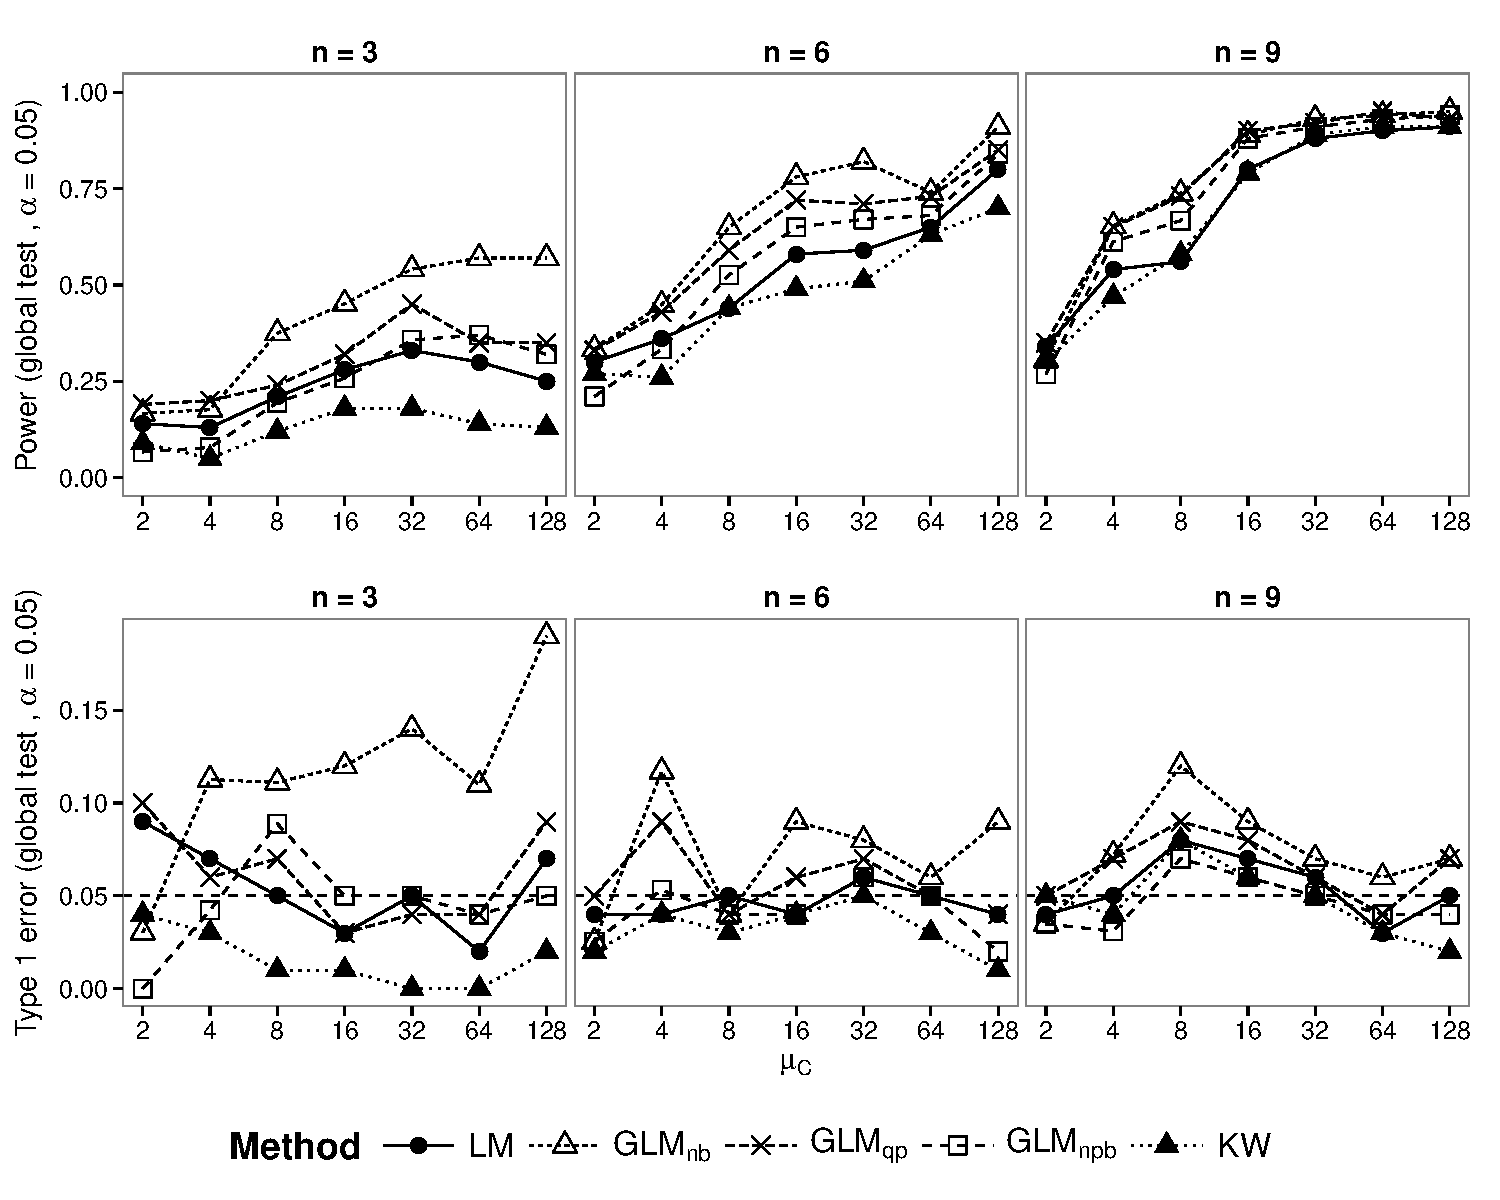
\includegraphics[width = 0.8\textwidth]{p_glob_c.pdf}
  \caption{Count data simulations: Power (top) and Type 1 error (bottom) for the test of a treatment effect.
  For n = 3 and $\mu_C$ = \{2, 4\} less than 80\% of $GLM_{nb}$ and $GLM_{npb}$ models did converge.
  Dashed horizontal line denotes the nominal Type 1 error rate at $\alpha = 0.05$.
  }
  \label{fig:p_glob_c}
\end{figure}

\begin{figure}
  \centering
  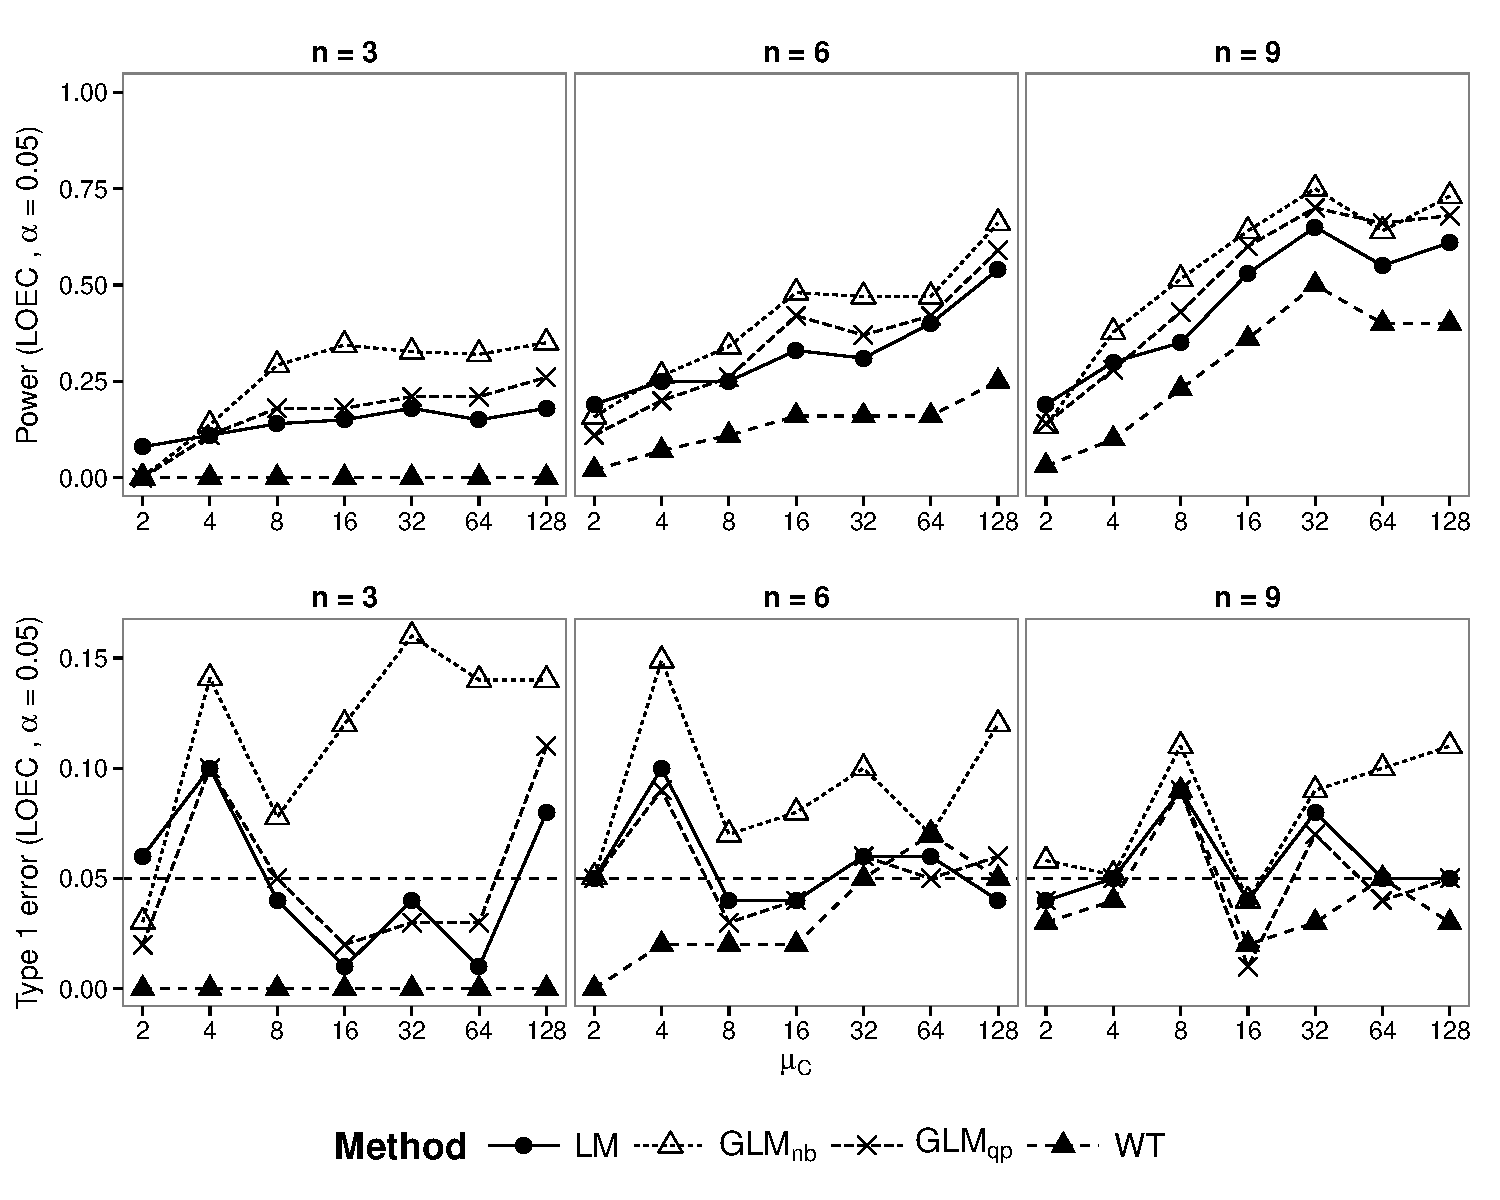
\includegraphics[width = 0.8\textwidth]{p_loec_c.pdf}
  \caption{Count data simulations: Power (top) and Type 1 error (bottom) for determination of LOEC.
  For n = 3 and $\mu_C$ = \{2, 4\} less than 80\% of $GLM_{nb}$ and $GLM_{npb}$ models did converge.
  Dashed horizontal line denotes the nominal Type 1 error rate at $\alpha = 0.05$.
  }
  \label{fig:p_loec_c}
\end{figure}


\subsubsection{Binomial data}
$GLM_{bin}$ showed the greatest power for testing the treatment effect. 
This was especially apparent at low sample sizes (n = 3), with up to 24\% higher power compared to LM.
KW had the lowest power and was slightly conservative.
However, the differences between methods quickly vanished with increasing samples sizes. 
KW was more conservative than LM and $GLM_{bin}$ (Figure \ref{fig:p_glob_p}).

Inference on LOEC was not as powerful as inference on the general treatment effect.
Contrary to the general treatment effect, $LM$ showed the higher power than $GLM_{bin}$ at small sample sizes.
However, these differences in power were only apparent at n = 3 and vanished quickly with increasing sample sizes (Figure \ref{fig:p_loec_p}). 
WT had no power for n = 3 and showed less power in the other simulation runs.
$LM$ maintained a Type 1 error level of 0.05 in all simulations. 
$GLM_{bin}$ was conservative at small effect sizes ($p_E > 0.8$) and WT was generally conservative showing lowered Type 1 error rates (Figure \ref{fig:p_loec_p}).

\begin{figure}
  \centering
  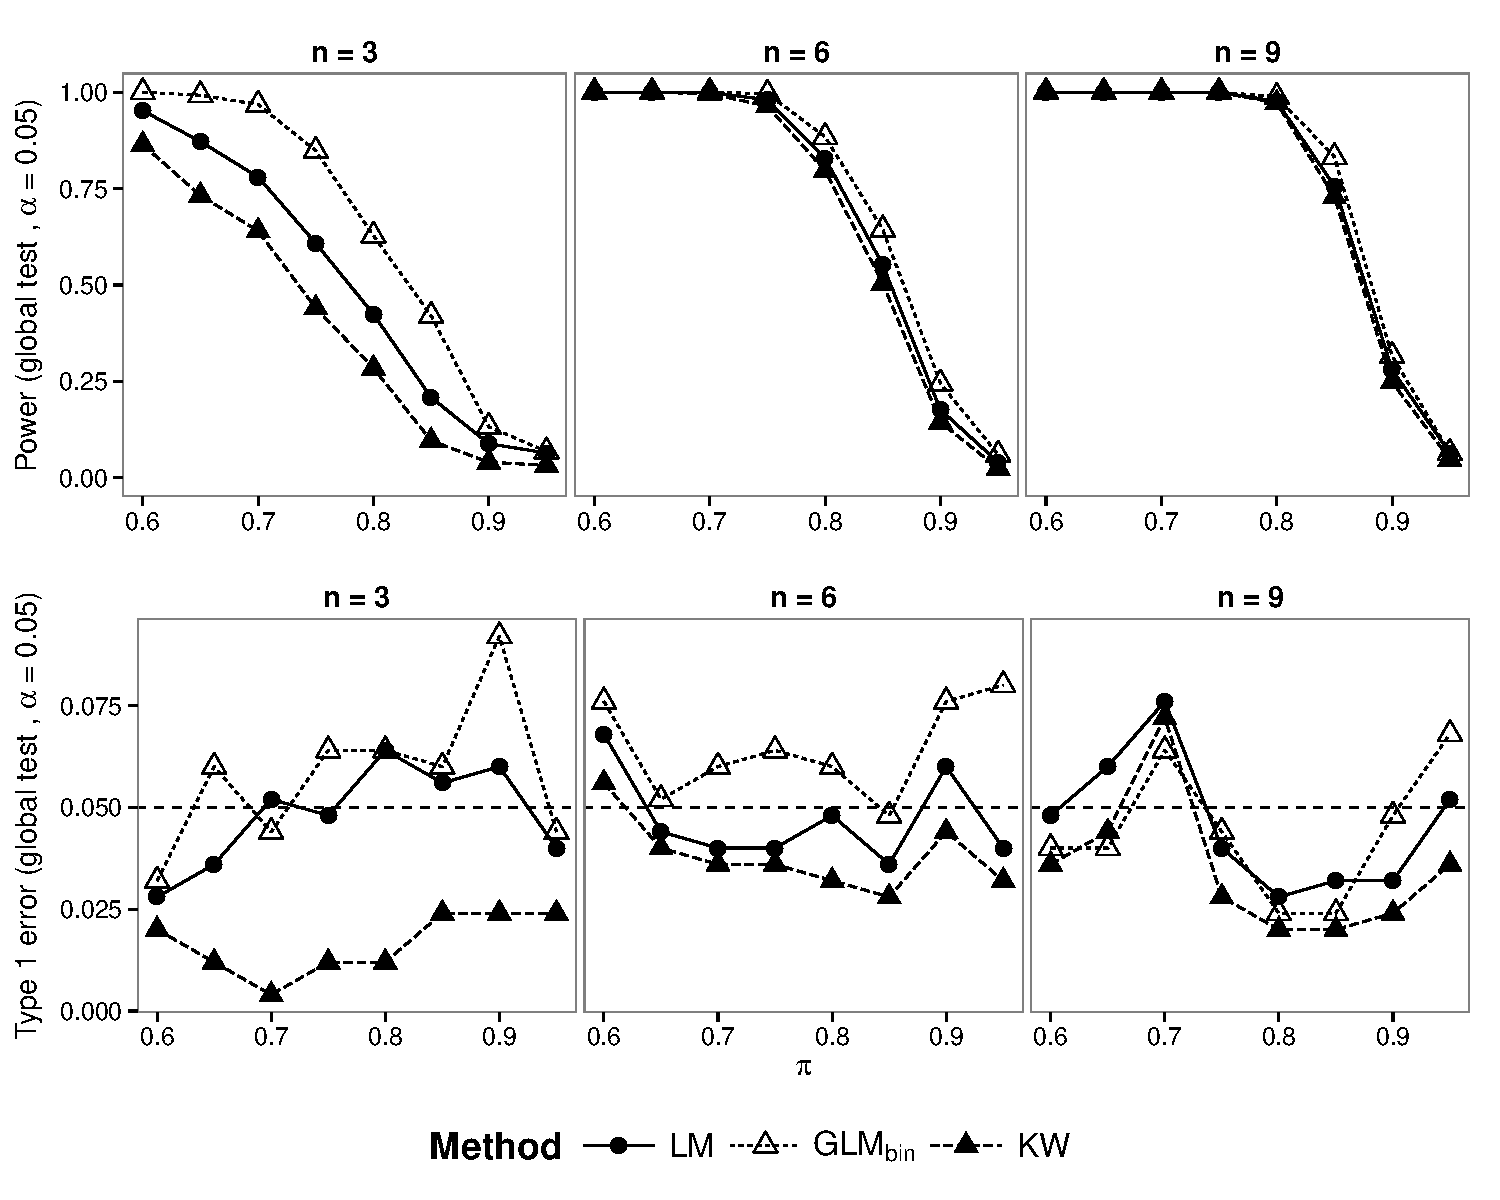
\includegraphics[width = 0.8\textwidth]{p_glob_p.pdf}
  \caption{
  Binomial data simulations: 
  Power (top) and Type 1 error (bottom) for the test of a treatment effect. 
  Dashed horizontal line denotes the nominal Type 1 error rate at $\alpha = 0.05$.
  }
  \label{fig:p_glob_p}
\end{figure}

\begin{figure}
  \centering
  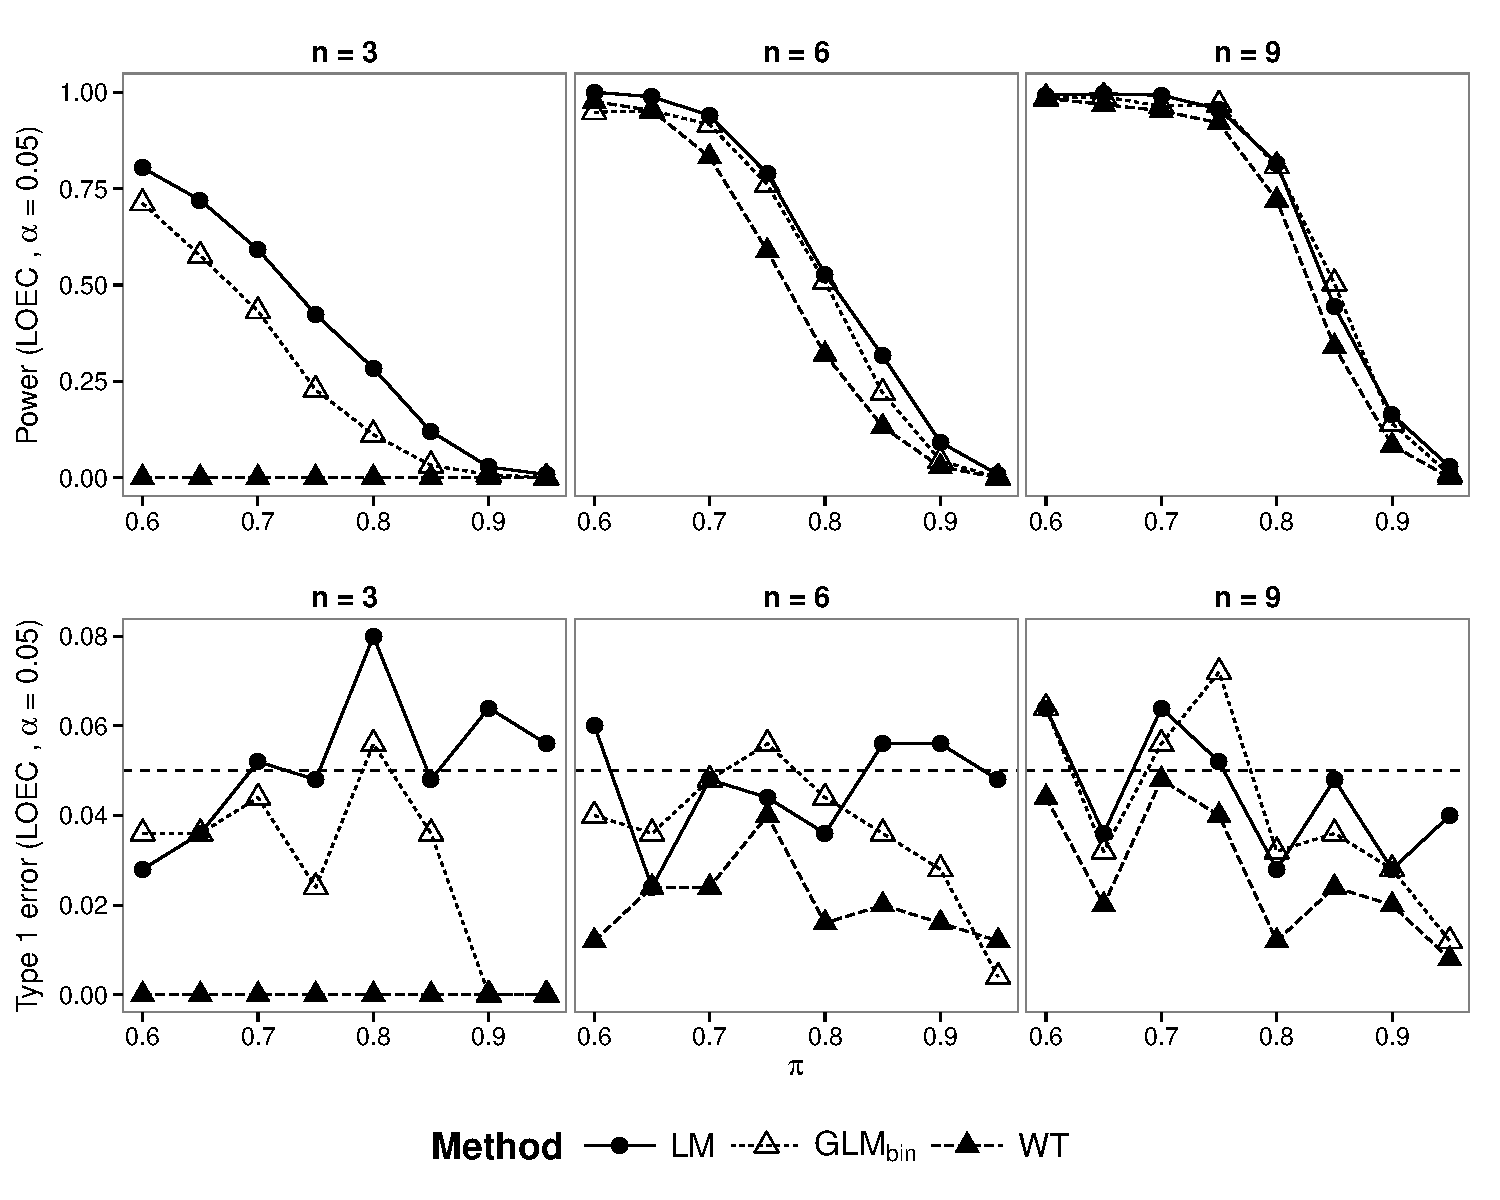
\includegraphics[width = 0.8\textwidth]{p_loec_p.pdf}
  \caption{
  Binomial data simulations: 
  Power (top) and Type 1 error (bottom) for the test for determination of LOEC. 
  Dashed horizontal line denotes the nominal Type 1 error rate at $\alpha = 0.05$.
  }
  \label{fig:p_loec_p}
\end{figure}


%% ----------------------------------------------------------------------------
\section{Discussion}
\label{sec:disc}
\subsection{Case study}
%% ---- Case study
The outlined case study demonstrates that the choice of the statistical model and procedure can have substantial impact on ecotoxicological inferences and endpoints like the LOEC.
This is further highlighted by the fact that for the same model (linear model of transformed data), \citet{brock_minimum_2015} reported a 10-fold lower LOEC (\mbox{0.3 mg/L}) then found in our study (3 mg/L, Figure \ref{fig:example}).
The reasons are be manifold: \citep{brock_minimum_2015} used a $log(2~y + 1)$ transformation, whereas we used a $log(A~y + 1)$ transformation, where A = 2 / 11 = 0.182 \citep{van_den_brink_impact_2000}.
Furthermore, \citet{brock_minimum_2015} used a one-sided Williams test which assumes a monotonic dose-response relationship.
In contrast, we used a one-sided Dunnett test, which does not assume monotonicity and allows individual comparisons between treatment groups and the control, but has under monotonicity less power \citep{jaki_statistical_2013}.


%% ---- Guide GLMs
Moreover, the case study illustrates the potential effects of overdispersion that is not accounted for: standard error will be underestimated and significance overestimated (Figure \ref{fig:example}).
However, in factorial designs the mean-variance relationship can be easily checked by plotting mean versus variance of the treatment groups (see supplemental material).
In the introduction we pointed out that there is little advice how to choose between the plenty of possible transformations - how do GLMs simplify this problem?
The distribution modelled can be chosen by the nature of the data giving a statistically sound model reflecting its properties (e.g. bonds, integer or continuous data etc.).
Knowing what type of data is modelled (see Methods section), the model selection process can be completely guided by the data and diagnostic plots. Therefore, choosing an appropriate model is more sound and straightforward than choosing between possible transformations.


\subsection{Simulations}
%% --- general low power
Our simulations showed that generally GLMs have greater power than data transformations.
However, the simulations also suggest that the power at the population level in common mesocosm experiments is low.
For common samples sizes and a reduction in abundance of 50\% we found a low power to detect any treatment-related effect (\textless 50\% for methods with appropriate Type 1 error, Figure \ref{fig:p_glob_c}).
Additionally, \citet{ohara_not_2010} showed that using a log transformation gave unreliable and biased parameter estimates.
Statistical power to detect the correct LOEC was even lower (less than 30\%).
This suggests that population level NOECs reported from mesocosm experiments should be interpreted with caution and underpins the criticism of NOEC \citep{laskowski_good_1995,landis_well_2011}.

%% --- Multivariate + GLMM -------
Mesocosm studies allow also inferences on community level. 
For community analyses \emph{GLM for multivariate data} have been proposed as alternative to Principal Response Curves (PRC) and yielded to similar inferences, but better indication of responsive taxa \citep{warton_distance-based_2012,szocs_analysing_2015}. 
Although our simulations covered only simple experimental designs at the population level, findings may also extend to more complex situations. 
Nested or repeated designs with non-normal data could be analysed using Generalised Linear Mixed Models (GLMM) and may have advantages with respect to power \citep{stroup_rethinking_2014}.

%% --- Alternatives -------
To counteract the problems with low power at the population level \citet{brock_minimum_2015} proposed to take the Minimum Detectable Difference (MDD), a method to assess statistical power \emph{a posteriori}, for inference into account.
However, \emph{a priory} power analyses can be performed easily using simulations, even for complex experimental designs \citep{johnson_power_2014}, and might help to design, interpret and evaluate ecotoxicological studies.
Moreover, \citet{brock_minimum_2015} proposed that statistical power of mesocosm experiments can be increased by reducing sampling variability through improved sampling techniques and quantification methods, though they also caution against depleting populations through more exhaustive sampling.
As we showed, using appropriate statistical methods (like GLMs) can enhance the power at no extra costs.

%% --- Non-parametric
\citet{wang_making_2011} advocated that in the typical case of small sample sizes (n \textless 20) and non-normal data, non-parametric tests perform better than parametric tests assuming normality.
In contrast, our results showed that the often applied Kruskal test and pairwise Wilcoxon test have equal or less power compared to tests assuming normality after data transformation.
Moreover, GLMs always performed better than non-parametric tests. 
Though more powerful non-parametric tests may be available \citep{konietschke_rank-based_2012}, these are focused on hypothesis testing and do not provide estimation of effect sizes.
Additionally to testing, GLMs allow the estimation and interpretation of effects that might not be statistically significant, but ecologically relevant.
Therefore, we advise using GLMs instead of non-parametric tests for non-normal data.

%% ---- Problems GLM
At small sample sizes and low abundances a significant amount of negative binomial models did not converge.
We used an iterative algorithm to fit these models \citep{venables_modern_2002} and other methods assessing the likelihood directly may perform better.
Moreover, the Likelihood-Ratio test gave an increased Type-I error for these models, where the non reliability of the LR statistic for small sample sizes has long been reported \citep{bolker_generalized_2009,wilks_large-sample_1938}. 
We found that parametric bootstrap ($GLM_{npb}$) provides a valuable alternative in such situations (Figure \ref{fig:p_glob_c}).
At small samples sizes, low abundances or few treatment groups it is difficult to determine the mean-variance relationship.
$GLM_{qp}$ assumes a simpler, linear mean-variance relationship, which might explain the higher power compared to $GLM_{npb}$ at small sample sizes (Figure \ref{fig:p_glob_c}, top).

%% --- binomial data
Binomial data is often collected in lab trials, where increasing the sample size is easy to accomplish. 
We found notable differences in power to detect a treatment effect up to a sample size of 9.
Similarly, \citet{warton_arcsine_2011} also found that GLM have higher power than arcsine transformed linear models.
Nevertheless, for deriving LOECs the transformation performed better at low sample sizes (n = 3) (Figure \ref{fig:p_loec_p}). 

We recommend that non-normal data should be analysed by GLMs and not by transformations or non-parametric methods.
To improve the power to detect effects, GLMs should become a standard method in ecotoxicology and incorporated into respective guidelines.



%% --------------------------------
\bibliography{references}
\bibliographystyle{apalike}

\end{document}
